%General
\documentclass{article}
\usepackage[utf8]{inputenc}
\usepackage{fullpage}

%Symbols
\usepackage{commath}
\usepackage{amsmath}
\usepackage{amssymb}
\usepackage{tikz}
\usetikzlibrary{arrows,automata}

\usepackage{listings}

\lstset{
  basicstyle=\itshape,
  xleftmargin=3em,
  literate={to}{$\rightarrow$}{2}
           {epsilon}{$\epsilon$}{1}
}

%Numbering
\usepackage{chngcntr}
\counterwithin{figure}{section}
\usepackage{enumerate}

%Formatting
\usepackage{bussproofs}
\usepackage{hyperref}
\usepackage{amsthm}
\usepackage{mathtools}
\usepackage{alltt}
\newtheorem{theorem}{Theorem}[section]
\newtheorem{definition}[theorem]{Definition}
\newtheorem{example}[theorem]{Example}
\hypersetup{colorlinks=true}
\hypersetup{colorlinks=true}
\usepackage{graphicx}
\graphicspath{ {img/} }
\usepackage{caption}

\title{Week 5: Context-free grammars}
\date{\today}
\author{Rikard Hjort}

\begin{document}
\maketitle

\section{}

Let $L$ be the language of the grammar. We wish to prove that for every element $w \in L$, the number of connectives is strictly smaller than the number of boolean constants. We prove this proposition through mathematical induction on the length of the derivation $B \xRightarrow{*} w$.

\begin{description}
    \item[Base case] Except for $B \to \mathsf{True}$ and $B \to \mathsf{False}$, no production rule yield a string consisting entirely of terminals, so only $\mathsf{True}$ and $\mathsf{False}$ can be constructed in a single derivation step, which is $B \Rightarrow \mathsf{True}$ or $B \Rightarrow \mathsf{False}$. In both these cases, the number of connectives in the string is 0, and the number of boolean constants is 1, so the proposition holds for derivations with one step.
    \item[Inductive step] We assume that the proposition holds for all derivations in $n$ steps or less. This is our inductive hypothesis, and we are thus using complete induction. Now suppose the derivation takes $n+1$ steps. Then the first derivation uses one of the five production rules, and then $n$ more steps. We shall prove in turn that whichever production rule we use for the first step of the derivation, the proposition holds.
        \begin{description}
            \item[$B \to B \lor B$:] The derivation of $w$ is $B \Rightarrow B \lor B \xRightarrow{*} w$. Now $w = x_1\lor x_2$ where $x_1 =\alpha_1...\alpha_k$ and $x_2=\alpha_{k+1}...\alpha_m$ are strings derived from $B$. Since all of $w$ is derived in $n+1$ steps, the derivation of both $x_1$ and $x_2$ must be in $n$ steps or less. Also, since $x_1$ and $x_2$ can both be derived from the starting symbol of the grammar, they are both in $L$. Call the number of constants in each of these substrings $t_1$ and $t_2$ respectively, and the number of connectives $s_1$ and $s_2$. Now, by the inductive hyposthesis, $t_1 > s_1 \Rightarrow t_1 \geq s_1+1$, and $t_2 > s_2 \Rightarrow t_2 \geq s_2+1$. Now the number of connectives in $w$ is $s_1 + 1 + s_2$ and the number of constants is $t_1 + t_2 \geq s_1 + 1 + s_2 + 1 = s_1 + s_2 + 2$, so $t_1 + t_2 > s_1 + s_2 + 1$, meaning the number of constants is strictly larger than the number of connectives.
            \item[$B \to B \land B$:] The proof for the case when the first step of the derivation uses this production rule is identical to the previous proof; one need only to replace all instances of '$\lor$' in the proof with '$\land$'.
            \item[$B\to(B)$] Since parentheses are neither constants nor connectives, the number of constants and connectives is the same as the numbers inside these outermost parentheses. Since the remainder of the derivation can be performed in $n$ steps, the number of constants in $w$ are strictly larger than the number of connectives, by the inductive hypothesis.
            \item[$B \to \mathsf{True}$ or $B \to \mathsf{False}$] The derivation ends after this step, $n+1 = 1$ and this is actually just the base case again.
        \end{description}
        
    \item[Conclusion] By the principle of strong induction, the proposition that the number of connectives is strictly smaller than the number of constants holds for all words in the language of the given grammar.
\end{description}


\newpage
\section{}

\begin{enumerate}[(a)]
    \item 
\begin{lstlisting}
A to aAd | B 
B to bBd | C 
C to cC | cD 
D to dD | epsilon
\end{lstlisting}

$A$ is the starting symbol.

    \item 
        To be a string in the language, a string must be made up of only a's followed by b's followed by c's followed by d's. The only restriction on the numbers of occurences of each letter is that the amount of d's must be at least as many as the a's and b's together. My grammar handles this by making sure that every time we add an a or a b, we must also add a d. At the end we can generate any number of d's, since there can be more d's than a's and b's together.

        I will also give a sligtly more formal proof.

    \begin{theorem} A word $w$ is in the given language if and only if it is generated by the grammar in (a).\end{theorem}
        \begin{proof}
        \end{proof}
        \begin{description}
            \item[If part] We generate a word from the grammar by applying the production rules. We start with $A$ and can choose between two production rules. We first apply the first production rule $i$ times, with $i \geq 0$, giving us the sentenial form $A \xRightarrow{*} a^iAd^i$. We then apply the second rule, giving us $A \xRightarrow{*} a^iBd^i$. From here, we only have variable $B$ to apply any rule to, and just like before, we apply the first rule $j$ times, $j \geq 0$, giving us $A \xRightarrow{*} a^ib^jBd^jd^i$. We then apply the second rule, giving us $A \xRightarrow{*} a^ib^jCd^jd^i$. We apply the first rule $k-1$ times, where $k-1 \geq 0$, giving $A \xRightarrow{*} a^ib^jc^{k-1}Cd^jd^i$. We then apply the second rule for $C$, yielding $A \xRightarrow{*} a^ib^jc^{k-1}cDd^jd^i$. Finally, we apply the first rule of $D$ $h - (i + j)$ times, with $h-(i+j) \geq 0$, and then the second rule, yielding $A \xRightarrow{*} a^ib^jc^{k-1}cd^{h-(i+j)}d^jd^i = a^ib^jc^kd^h$. 

                Looking at the construction of the string we notice that this describes all possible productions we can do. The first rule of each variable can be used an arbitrary number of times, since it is recursive. We can choose it as many times as we like, including 0 times. Since it only contains one variable, each invocation lets us choose production one more time. As soon as we pick the second rule, we "move on" to the next variable, or terminate in the case of $D$.

                We also notice that $i, j \geq 0$, that $k-1 \geq 0 \Rightarrow k > 0$, and that $h -(i + j) \geq 0 \Rightarrow h \geq i+j$. Whichever number of invocations of each rule we choose to do, the form of the resulting string we guarantee that it is in the language.
            \item[Only-if part] Given any string in the language, we can repeat the process above, using the values of the exponents in exactly the same manner as they were used above. We will then follow a complete derivation of a string from the starting symbol, and the string will be generated by our grammar.
        \end{description}
    \item No. Every symbol can only have been generated by a certain production rule. All a's come from A, all b's from B, all c's from C, and always get added from the left. d's are created by A and B at first, which each d corresponding to the a or b at the mirrored position. When there are no mirroring a's or b's, the d is created by D.

        Another way to put it is to look at the final string of the derivation: $A \xRightarrow{*} a^ib^jc^{k-1}cd^{h-(i+j)}d^jd^i $. All the symbols belonging to an $i$-exponent were generated in the first rule of $A$, every belonging to a $j$ exponent in the first rule of $B$, every symbol beloning to a $k-1$ exponent from the first rule of $C$, and so on. Thus, for any string in the language, every character can only come from one production rule. Furthermore, each production rule must be repeated an exact number of times, as seen above, and they must be done in sequence. If we choose a different production rule at any time than prescribed by the algorithm above, we can never "return" and finish the job of that rule, which is to add more of a certain symbol. And since there is only one variable available in every step of the derivation, all derivations are both leftmost and rightmost derivations. Since there is only on possible leftmost derivation for each string, the grammar is unambiguos.

    \item

        \begin{description}
            \item[Recursive inference]

        We begin by assigning a number to every production of the grammar:

\begin{lstlisting}
1. A to aAd
2. A to B 
3. B to bBd
4. B to C 
5. C to cC 
6. C to cD 
7. D to dD
8. D to epsilon
\end{lstlisting}

                We will then write the recursive inference in the form of a table, in the same manner as in chapter 5 of the course book.

                $$
                \begin{array}{l | l | l | l | l}
                    & \text{String inferred} & \text{For languages of }& \text{Production used }& \text{Strings(s) used} \\ \hline \hline
                    (i) & \epsilon & D & 8 & – \\
                    (ii) & d & D & 7 & (i) \\
                    (iii) & cd & C & 6 & (ii) \\
                    (iv) & cd & B & 4 & (iii) \\
                    (v) & bcdd & B & 3 & (iv) \\
                    (vi) & bcdd & A & 2 & (v) \\
                    (vii) & abcddd & A & 1 & (vi)
                \end{array}
                $$
            Since $A$ is the starting symbol of the grammar, and $abcddd$ is in the language of $A$, $abcddd$ is generated by the grammar.
            
            \item[Leftmost derivation]
                \begin{align*}
                    &A \xRightarrow[lm]{} aAd \xRightarrow[lm]{} aBd \xRightarrow[lm]{} abBdd \xRightarrow[lm]{} abCdd \xRightarrow[lm]{} \\
                    &abcDdd \xRightarrow[lm]{} abcdDdd \xRightarrow[lm]{}
abcddd
                \end{align*}

            \item[Parse tree] The parse tree is given in figure \ref{fig:parse} 
                \begin{figure}[htpb]
                    \centering
                    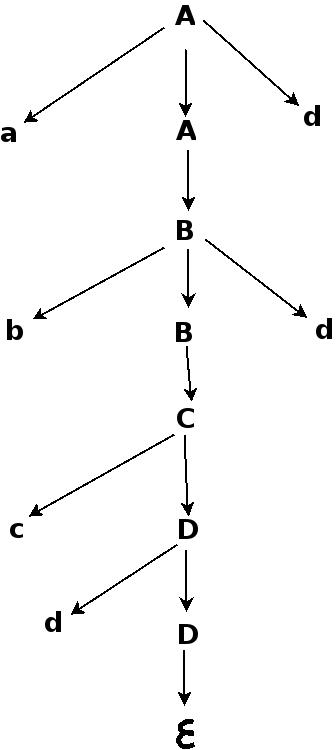
\includegraphics[width=0.15\linewidth]{parse}
                    \caption{The parse tree of the string $abcdd$ in the grammar.}
                    \label{fig:parse}
                \end{figure}
        \end{description}
\end{enumerate}

\newpage
\section{}

\begin{enumerate}[(a)]
    \item The language of $B$ is all strings of one or more 1's. The language of $A$ is all strings of one or more 0's, suffixed by the language of $B$. So the language of $A$ is all strings of one or more 0's followed by one or more 1's. From the start variable we can generate the language of $A$, and also surround it with any number of leading 0's and trailing 1's, which still gives us the language of all strings of one or more 0's followed by one or more 1's.
        
        Using set notation, the language of $S$, and thus the language of the grammar, is $\set{0^n1^m | n,m > 0}$. We will call this language $L$.

    \item Take the string $0011$. It can be created by the leftmost derivation

        \begin{align*}
            S \xRightarrow[lm]{} 0S1 \xRightarrow[lm]{} 0A1 \xRightarrow[lm]{} 00B1 \xRightarrow[lm]{} 0011
        \end{align*}

        or by the leftmost derivation 

        \begin{align*}
            S \xRightarrow[lm]{} A \xRightarrow[lm]{} 0A \xRightarrow[lm]{} 00B \xRightarrow[lm]{} 001B \xRightarrow[lm]{} 0011
        \end{align*}

        Since these are two distinct leftmost derivations – for example, the first production rule used differs – they would generate different parse trees, and the grammar is thus ambiguos.

    \item
        We hinted at this in (a). The language of $A$ is the same as the language of $S$, so we need only to create a grammar that is like the one given, only the variable $S$ and all its productions are removed, and we make $A$ the start symbol.

        \begin{lstlisting}
        A to 0A | 0B 
        B to 1B | 1 
        \end{lstlisting}

        $A$ is the start symbol.

    \item
        We have only 4 production rules. For any string in the language, the rightmost 0 must have been produced by the second rule of A, and all other 0's must have been produced by the first rule of A. All 1's except the last one must have been produced by the second rule of B, and the rest by the first rule of B. Thus for any given string $0^n1^m$ in the language, there is only one choiche of derivation:
        \begin{enumerate}[(1)]
            \item Starting with $A$, use the rule $A \to 0A$ $n-1$ times.
            \item Use the rule $A \to 0B$.
            \item Use the rule $B \to 1B$ $m-1$ times.
            \item Use the rule $B \to 1$.
        \end{enumerate}

        If we use $A \to 0B$ before using $A \to 0A$ $n-1$ times, we will have a sentenial form with less than $n$ 0's followed by a $B$. From here, no production rule allows anything else than adding 1's, so we will have less than $n$ 0's. The same reasoning applies for if we try to use the rule $B \to 1B$ less than $m-1$ times. 
        
        Conversely, if we use any of the recursive rules more than $n-1$ times or $m-1$ times respectively, we will end up with more than $n$ 0's or more than $m$ 1's, so then it is not the required string. So there is only one leftmost derivation possible for the string\footnote{Actually, since every rule contains 1 variable or less, the leftmost derivation, the rightmost derivation and every other derivation is the same.}.
\end{enumerate}

\end{document}
